\documentclass{article}

% ===== Graphics =====
\usepackage{graphicx}
\usepackage{svg}
\graphicspath{{resources/}}

% ===== Colors =====
\usepackage{xcolor}
\definecolor{darkergray}{gray}{0.25}

% ===== Page layout =====
\usepackage[
letterpaper,
top=2.5cm,
bottom=2.5cm,
left=1.5cm,
right=1.5cm,
columnsep=20pt
]{geometry}


% ===== Bibliography with biblatex =====
\usepackage[
backend=biber,
style=numeric,
sorting=none
]{biblatex}
\addbibresource{resources/bibliography.bib} % <-- your .bib file location

\renewcommand*{\bibfont}{\footnotesize}  % Very small font
\setlength{\bibitemsep}{0.25em}         % Tight spacing

% ===== Other styling =====
\usepackage{parskip}    % no indentation, space between paragraphs
\usepackage{titlesec}   % custom section titles
\usepackage{amsmath}
\usepackage{ragged2e}   % for \justifying
\usepackage{microtype}  % better typography
\usepackage{hyperref}   % hyperlinks
\usepackage{float}
\usepackage{paralist}
\usepackage{placeins}
\usepackage{balance}



% ===== Justification and bad box fixes =====
\AtBeginDocument{\justifying}
\sloppy
\setlength{\RaggedRightRightskip}{0pt plus 0.1\textwidth}

% ===== Section title formatting =====
\titleformat{\section}
{\normalfont\large\bfseries\centering\MakeUppercase}
{\thesection.}{1em}{}
\titleformat{\subsection}
{\normalfont\large\bfseries\centering\MakeUppercase}
{\thesubsection.}{1em}{}

\titlespacing*{\section}{0pt}{3.25ex plus 1ex minus .2ex}{1.5ex plus .2ex}
\titlespacing*{\subsection}{0pt}{3.25ex plus 1ex minus .2ex}{1.5ex plus .2ex}

% ===== Document metadata =====
\title{Mapping National AI Research Authority through Subdisciplinary Differentiation: A Scientometric Study Using OpenAlex (2020–2025)}
\author{Julius Pfundstein \\[1em]
	University of Leipzig \\
	Digital Humanities \\
	julius.pfundstein@studserv.uni-leipzig.de}
\date{Oktober 2025}

\begin{document}

\color{darkergray}


\begin{titlepage}
	
	\vspace*{1cm}
	\centering
	{\LARGE\bfseries Mapping National Artificial Intelligence Research Authority\par}
	\vspace{1em}
	{\LARGE\bfseries A Scientometric Analysis of AI Subdisciplines Using OpenAlex (2020–2025)\par}
	\vspace{3cm}

    {\large
             Julius Pfundstein \\ \vspace{2em}
             Faculty of Mathematics and Computer Science \\ \vspace{2em}
             University of Leipzig \\ \vspace{2em}
             julius.pfundstein@studserv.uni-leipzig.de \par}
    
    % Logo section
    \vspace{3cm}
		
\includegraphics[height=3cm, keepaspectratio]{university_of_leipzig_logo.pdf} % Fixed height of 
    
    % Date section
    \vspace{3cm}  % Space between logo and date
    {\large Oktober 2025 \par}
    
    \vfill
    \thispagestyle{empty}
\end{titlepage}

\cleardoublepage
\thispagestyle{empty}

\vspace*{4cm}

\begin{center}
	\Huge\textbf{Acknowledgments}
\end{center}

\vspace{2cm}

\noindent
I would like to express my deepest gratitude to my supervisor,\\
\textbf{Dr. Thomas Efer},\\
for his invaluable guidance, continuous support, and insightful feedback throughout the course of my master’s thesis.

\vspace{1cm}

\noindent
I also wish to sincerely thank the OpenAlex team for generously providing access to their API, which enabled the extensive data collection and analysis crucial to this research.

\vspace{3cm}

\noindent
\textbf{Faculty of Mathematics and Informatics}\\
\textbf{University of Leipzig}\\
\textbf{Master of Science in Digital Humanities}

\vfill


\newpage

\vspace*{4cm}

\begin{abstract}
	
	Artificial intelligence (AI) has rapidly emerged as a foundational general-purpose technology, profoundly reshaping productivity across multiple sectors including manufacturing, services, healthcare, finance, and defense. Beyond optimizing discrete tasks, AI increasingly reconfigures the institutional and geopolitical frameworks through which knowledge, value, and power are produced and contested. This raises critical questions about the distribution of technological authority within the global AI research ecosystem.
	
	This study addresses two central research questions: (1) Which subdisciplines compose the contemporary field of AI research? and (2) How are countries and regions positioned within these subfields in terms of research capacity and influence? Utilizing a comprehensive dataset of over three million AI-related publications from OpenAlex, we implement hierarchical topic modeling on titles and abstracts to delineate distinct AI subdisciplines. We then apply citation network analysis to measure the relative centrality and scholarly impact of countries within each subfield.
	
	By integrating thematic and network-based bibliometric methods, this work offers a detailed, subdiscipline-specific mapping of the global AI research landscape. The findings illuminate the complex structure of AI as a multifaceted domain and reveal the geographic patterns of research leadership, providing a critical empirical foundation for understanding the evolving loci of AI-driven power and influence.
	

\end{abstract}

\vspace{2cm} % extra space between abstract and keywords

\begin{flushleft}

\hspace*{1cm}\textbf{Keywords:} Artificial Intelligence, Bibliometrics, Scientometrics, Global AI Research, Country Ranking



\end{flushleft}

\newpage

\tableofcontents
\thispagestyle{empty}
\newpage

\pagenumbering{arabic}

\twocolumn

\section{Introduction}

Artificial intelligence has emerged as a general-purpose technology, woven deeply into the fabric of contemporary productivity. Much like the electrification of industry once redefined the foundations of economic growth, AI now underpins advances across manufacturing \cite{kim2022recent}, services \cite{huang2018artificial}, healthcare \cite{alkuwaiti2023review}, finance \cite{bahoo2024artificial}, and defense \cite{sabouri2024newgeopolitics} \cite{vance2023geopolitical}. Its pervasive integration means that AI does not merely optimize isolated tasks but increasingly conditions the structures through which knowledge, value, and strategic advantage are generated and contested. Technologies of such systemic importance inevitably transcend the technical; they become instruments through which power is organized, exercised, and shifted within and between states.

For political science, this raises an enduring yet newly urgent inquiry: \emph{where does the power embedded in this technological capacity reside, and how is it distributed across the globe?}

Addressing such questions empirically calls for tools capable of systematically tracing patterns of knowledge production, diffusion, and influence across large-scale scientific activity. Scientometrics, as the quantitative study of science and scholarly communication, provides a robust framework for capturing these dynamics by analyzing publication data, citation networks, and thematic structures within research fields.

A review of the existing literature reveals substantial efforts to map the global landscape of artificial intelligence research. This body of work has produced valuable insights into national capacities, collaboration patterns, and knowledge flows. However, much of this research remains limited in at least one of five critical respects:
\begin{enumerate}
	\item Analyses relying on outdated data fail to capture recent developments and dynamics within the field. \cite{niu2016global}
	\item Studies with narrow application focus—such as AI in life sciences \cite{schmallenbach2024global} or innovation \cite{mariani2023artificial}—neglect the comprehensive disciplinary structure.
	\item Conceptualizing AI as a unified domain obscures the heterogeneity of subfields characterized by distinct methodologies and strategic priorities. \cite{almarzouqi2024comparative,cao2020international, vinayak2023signatures, alshebli2022beijing, hu2020global}
	\item Scientometric analyses that prioritize authorship-level metrics lack systematic evaluation of national and regional research positioning.
	\item National AI capacity assessments typically exclude multi-dimensional benchmarking frameworks beyond scientometric indicators. \cite{ozkaya2023analysis}
\end{enumerate}



Taken together, these limitations illustrate why existing work remains insufficient for capturing the full scope and complexity of contemporary artificial intelligence research. Analyses constrained by outdated data, narrow disciplinary scope, or overly aggregated concepts risk masking the field’s internal differentiation and its shifting centers of expertise. Likewise, a sole focus on authorship-level patterns or on single indicators overlooks the multiple scales and dimensions through which technological capacity is organized and expressed. Addressing these gaps requires an approach that combines fine-grained topical resolution with systematic, comparative assessment at the country level.


To address this limitation, two guiding research questions structure the present analysis:

\begin{enumerate}
	\item[\textbf{RQ1}] \emph{Which subdisciplines structure the contemporary field of artificial intelligence research?}
	\item[\textbf{RQ2}] \emph{How are countries and regions positioned within these subdisciplines in terms of their relative research capacity and influence?}
\end{enumerate}

These questions serve as the foundation for the empirical strategy and frame the subsequent analysis.


To address these research questions, this study utilizes a comprehensive dataset comprising over three million artificial intelligence research publications sourced from OpenAlex. \cite{openalex2023} A hierarchical topic modeling approach is applied to the titles and abstracts to identify and characterize the distinct subdisciplines within AI. Subsequently, a citation network analysis quantifies the relative centrality and influence of countries and regions within these identified subfields. This combined methodology enables a nuanced mapping of the global AI research landscape, providing empirical insight into both the internal structure of AI as a research domain and the geographic distribution of scholarly leadership.

\section{Research Review}

The global distribution of research capacities in artificial intelligence has attracted increasing scholarly and policy attention in recent years. Numerous studies have examined national investments, scientific output, and patterns of collaboration in AI-related fields, reflecting concerns about technological leadership, economic competitiveness, and strategic autonomy \cite{REF}. Comparative assessments often rely on publication counts, patent registrations, or research funding indicators to measure countries’ positions within the global AI landscape \cite{REF}.

This body of work has provided valuable insights into the dynamics of knowledge production, the role of leading institutions, and the emergence of new centers of AI expertise \cite{REF}. However, a common limitation of many large-scale comparative studies is their tendency to treat artificial intelligence as a single, unified domain. Such an approach risks masking substantial heterogeneity within AI, which spans diverse technical domains, application areas, and research communities. Recent contributions have begun to recognize this internal diversity, for example by mapping thematic clusters or tracing the evolution of specific subfields such as deep learning or natural language processing \cite{REF}. Nevertheless, systematic and scalable analyses that combine topic modeling with cross-national comparison remain limited.

In addition to thematic differentiation, the question of scientific influence and leadership is often approached through simple output metrics, such as publication counts or citation aggregates at the national level. While these measures capture research volume, they can obscure structural aspects of influence within scientific networks. Network-based indicators — such as citation centrality — offer a more nuanced perspective by highlighting how ideas, methods, and findings diffuse and concentrate across communities \cite{REF}.

Against this backdrop, the present study aims to contribute to the literature by systematically disaggregating the AI research domain into empirically derived subdisciplines and situating countries within these subfields based on their structural position in global citation networks. This approach complements existing work by combining large-scale topic modeling and network analysis to capture both the thematic complexity of AI and the relational dynamics that underpin scientific leadership.


\section{Data}


This chapter outlines the systematic approach undertaken to assemble a robust and representative dataset of artificial intelligence research publications. It begins by discussing the selection criteria for the underlying scientific knowledge graph, followed by the construction of a comprehensive search query based on an extensive review of recent AI survey literature. Subsequent sections detail the data retrieval process, post-processing steps including duplicate removal and metadata validation, and the preparation of the final corpus for analysis. This structured approach ensures that the dataset aligns closely with the study’s objectives and provides a reliable foundation for the applied topic modeling and citation network methods.

\subsection{SKG-Comparison}

Analyses of technological capacity and leadership often rely on empirical indicators such as economic output, patent filings, or scientific publications. While economic and patent data capture dimensions of technological application and commercialization, they offer only limited insight into the underlying processes of knowledge generation and scholarly exchange that drive emerging research frontiers. In the context of artificial intelligence — a domain where conceptual advances and methodological innovations are tightly interwoven with practical applications — peer-reviewed research outputs provide a particularly suitable proxy. Scientific publications document not only the scale of research activity but also its thematic orientation, methodological diversity, and the collaborative structures through which knowledge is produced and diffused.

To examine these dynamics systematically, this study employs OpenAlex as the principal data source. OpenAlex belongs to the class of Scientific Knowledge Graphs (SKGs), which integrate scholarly metadata, citation relationships, institutional affiliations, and research topics into structured, interlinked databases. Prominent SKGs include Web of Science, Scopus, and Microsoft Academic Graph (MAG). Compared to proprietary platforms, OpenAlex offers broader disciplinary coverage, strong representation of recent and interdisciplinary works, and open programmatic access that supports scalable, reproducible analysis. 

A comparative overview of leading SKGs is provided in Table~\ref{tab:skg_comparison}, highlighting the features that make OpenAlex particularly well suited to address the present research questions concerning thematic differentiation and network-based measures of scholarly influence.


\begin{table*}[t]
	\centering
	\caption{Comparison of Major Scientific Knowledge Graphs}
	\label{tab:skg_comparison}
	\small
	\begin{tabular}{lcccc}
		\hline
		\textbf{Metric} & \textbf{Web of Science} & \textbf{Scopus} & \textbf{Dimensions} & \textbf{OpenAlex} \\
		\hline
		\textbf{Basic Coverage} & & & & \\
		Total documents (millions) & 90 & 94 & 134 & 248 \\
		\hline
		\textbf{Metadata Completeness} & & & & \\
		DOI coverage & 98\% & 97\% & 95\% & 99\% \\
		Author ORCID linkage & Partial & Yes & Yes & Yes \\
		Abstract availability & High & High & High & High \\
		Referenced works coverage & High & High & High & High \\
		Citation count availability & High & High & High & High \\
		\hline
		\textbf{Geographic Coverage} & & & & \\
		English-language dominance & High & High & Moderate & Low \\
		Non-English abstracts & 15\% & 25\% & 30\% & 40\% \\
		Developing country coverage & Moderate & Good & Excellent & Good \\
		\hline
		\textbf{Access \& Features} & & & & \\
		API access & Restricted & Restricted & Full & Full \\
		Open access & No & No & Partial & Yes \\
		Cost model & Subscription & Subscription & Freemium & Free \\
		Text mining allowed & Limited & Limited & Yes & Yes \\
		\hline
	\end{tabular}
	
	\vspace{2.5em}
	{\footnotesize
\textbf{Note:} The data presented in this table reflect the state of the respective scientific knowledge graph platforms as closely as possible to the time of dataset compilation in June 2025. Given the dynamic and continuously evolving nature of these resources, values may be subject to temporal variation and periodic updates.
	}
\end{table*}


Among the available Scientific Knowledge Graphs, OpenAlex offers specific advantages that align closely with the analytical goals of this study. Unlike many proprietary databases that prioritize indexing high-impact journals and rely on selective curation, OpenAlex adopts an inclusive indexing strategy that reduces coverage bias toward established or elite institutions. This broader scope enhances the visibility of contributions from emerging research contexts, including non-OECD countries and institutions outside traditional centers of scientific production.

Moreover, OpenAlex provides the strongest representation of non-English language outputs among major SKGs, which is critical for capturing regional and national specializations that may be underrepresented in predominantly Anglophone collections. Its comprehensive metadata — including consistent DOI assignment, author identifiers, abstracts, referenced works, and citation counts — ensures the completeness and comparability required for robust topic modeling and network analysis.

Finally, OpenAlex’s open-access licensing and unrestricted API facilitate scalable data collection and reproducibility, both of which are essential for large-scale scientometric studies. Taken together, these characteristics position OpenAlex as the most suitable source for examining the internal structure of artificial intelligence research and the relative standing of countries within this dynamically evolving field.

It must be acknowledged, however, that all Scientific Knowledge Graphs, including OpenAlex, reflect inherent biases related to language, regional publishing practices, and coverage policies. Recent comparative assessments (e.g., \cite{REE}) have highlighted systematic differences across SKGs that can shape analytical outcomes. Recognizing these limitations is essential for interpreting the results presented in this study.


\subsection{Extraction Pipeline}


\clearpage
\onecolumn          % leave two-column mode
\begin{center}
	{\large\textbf{Figure~\ref{fig:log_bar_graph}: Dataset Construction Pipeline Diagram}}
	\vspace{1em}
\end{center}

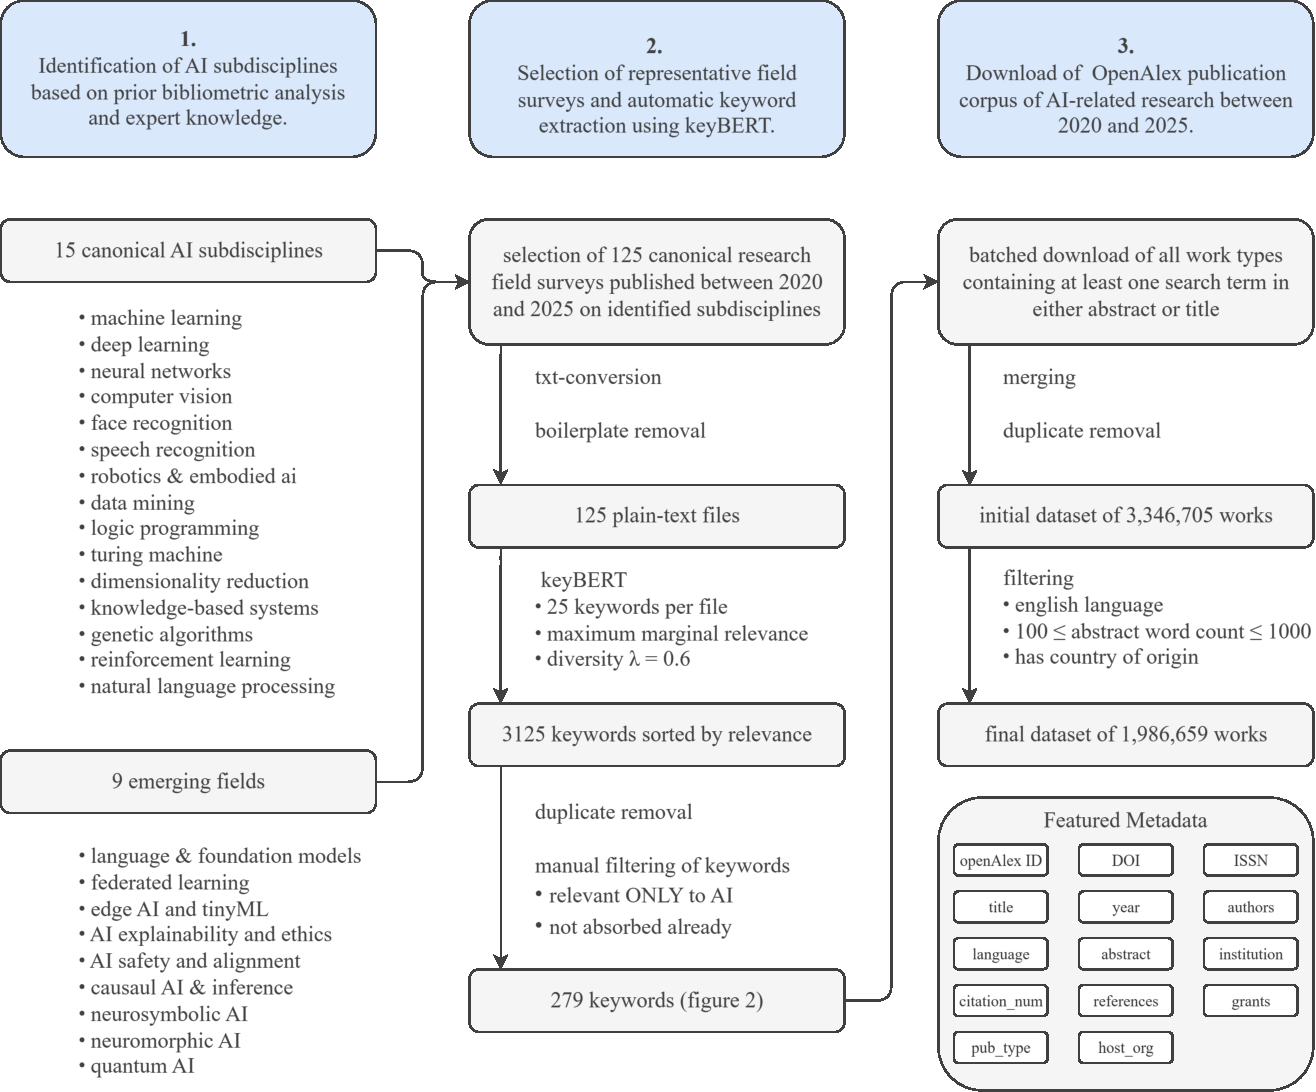
\includegraphics[width=\textwidth]{data_extraction_pipeline_diagram.pdf}
\label{fig:log_bar_graph}

\twocolumn          % return to two-column mode




\subsection*{Extraction Pipeline}

The selection of publications is a crucial determinant of this study’s analytical validity. As Baruffaldi et al. propose, building a comprehensive query for artificial intelligence research requires a structured keyword set; their 2020 study derived a list of 193 AI-related terms from AI-labeled publications from Scopus. \cite{baruffaldi2020identifying} However, given the rapid evolution of the field, such a list must be continuously revised to reflect emerging subdisciplines and novel applications. To address this, a similar but updated approach was undertaken here. The extraction process began with a framework established by Gargiulo et al.\ \cite{gargiulo2022cartography}, who applied topic modeling to delineate 15 principal AI subfields that collectively define the core technological landscape. These subfields form the initial structure for constructing a refined and thematically precise search strategy, which is detailed in the following sections.


\begin{inparaenum}[(1)]
	\item Neural networks,
	\item deep learning,
	\item machine learning,
	\item reinforcement learning,
	\item natural language processing,
	\item computer vision,
	\item face recognition,
	\item speech recognition,
	\item robotics,
	\item data mining,
	\item logic programming,
	\item Turing machines,
	\item dimensionality reduction,
	\item expert systems,
	\item and genetic algorithms.
\end{inparaenum}


Building on this taxonomy, an intensive literature review identified an additional nine emergent subdisciplines that have gained significant attention post-2022, reflecting the rapid evolution of AI research. These include, among others, 
\begin{inparaenum}[(1)]
	\setcounter{enumi}{15} % continues numbering from your previous 15 items
	\item language models and foundation models,
	\item federated learning,
	\item edge AI,
	\item AI explainability and ethics,
	\item AI safety and alignment,
	\item causal AI,
	\item neurosymbolic AI,
	\item neuromorphic AI,
	\item and quantum AI.
\end{inparaenum}

For each identified subdiscipline, a corpus of survey papers was assembled, restricted to publications from 2019 onward to ensure topical relevance. Survey papers were selected because they offer comprehensive overviews of their respective fields, cite a wide range of seminal works, and avoid overly specialized or niche vocabulary that might exclude broader field indicators. In total, 125 survey papers were collected.

From these survey papers, keywords were extracted using a modified version of the KeyBERT algorithm. This approach yielded an initial set of 3,175 candidate keywords, which underwent manual refinement to isolate the 279 terms most exclusively relevant to artificial intelligence research. This refined keyword list served as the basis for constructing the search query applied to the OpenAlex database.

A simplistic keyword query such as ``Artificial Intelligence'' was initially tested but proved insufficient. An exact keyword match on titles and abstracts returned only approximately 570{,}714 works, many of which were tangential to the technological aspects of AI. Analysis of OpenAlex-provided concept distributions in a random sample of 10{,}000 works revealed that a substantial fraction pertained to non-technical domains, including economics (3.0\%), political science (2.3\%), law (2.2\%), sociology (1.0\%), and philosophy (0.9\%). While these areas offer valuable perspectives, the focus of this study on technological capacities necessitated minimizing their representation to enhance precision without sacrificing recall.

To further address this challenge, the final keyword set deliberately excludes certain broad or cross-disciplinary concepts---such as \textit{multi-agent systems}, \textit{natural language processing}, \textit{genetic algorithms}, and \textit{expert systems}---which, despite their centrality within AI, also have substantial relevance in other domains that could introduce thematic noise and inflate the dataset with unrelated documents. Likewise, generic umbrella terms like \textit{artificial intelligence} itself were omitted for the same reason: they frequently appear in social science publications that seek to contextualize the phenomenon rather than contribute to its technical development. Acronyms such as \textit{GAN}, \textit{CNN}, \textit{RLHF}, \textit{GNN}, and \textit{SNN} were also excluded, as they often have multiple domain-specific meanings and can generate ambiguous matches, particularly given that the search is case-insensitive and abbreviations can appear embedded within unrelated words (for instance, \textit{RAG} in \textit{fragmentation}). Even the standalone term \textit{AI} was omitted except when paired with additional descriptors that unambiguously anchor it within computer science.

Conversely, some keywords were retained in the final list even though they cannot be exclusively attributed to AI research. For instance, methods such as \textit{backpropagation} or \textit{random forest} are also widely used in broader statistical learning and other related fields. However, given their strong association with AI-driven machine learning tasks, it was assumed that their inclusion would primarily yield AI-relevant publications, thus justifying their retention. By contrast, terms for which a clear or probable secondary meaning exists---such as \textit{BERT} or \textit{PaLM}---were excluded to minimize ambiguity and unintended retrieval.

This cautious curation ensures that the resulting corpus remains as technically focused as possible while minimizing false positives. Consequently, the comprehensive keyword list was constructed with the dual objective of maximizing recall for AI-relevant publications and minimizing the inclusion of unrelated works. The list was implemented in a Boolean \texttt{OR} query to retrieve a broad yet targeted dataset for subsequent analysis.

A visualization of the number of retrieved results per individual search term is provided in Figure~\ref{fig:log_bar_graph}. The fact that the total number of retrieved documents falls short of the sum of the individual term results is explained by the overlap inherent in the query design: multiple search terms frequently co-occur in the title and abstract of a single document.

\begin{figure*}[!p]
	\centering
	\caption{Logarithmic bar graph of retrieval count per search term}
	\vspace{1em}
	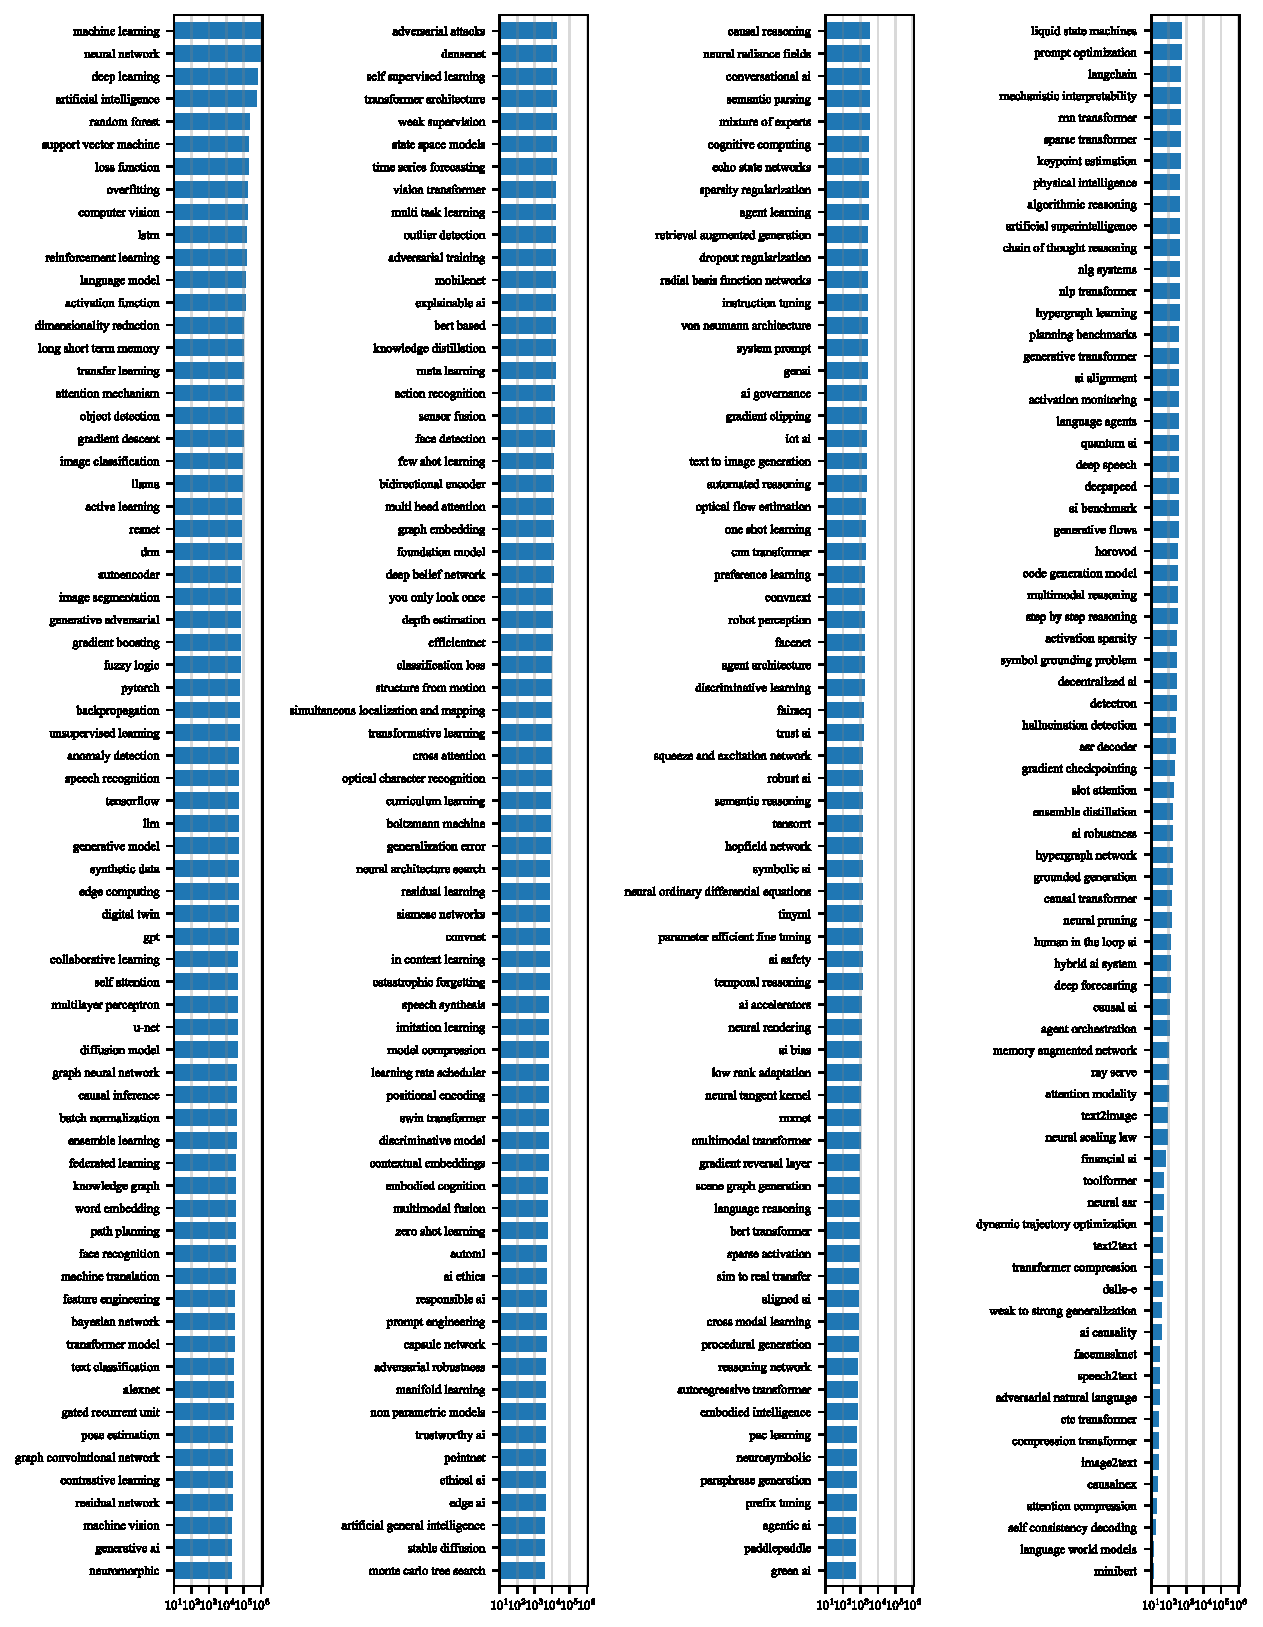
\includegraphics[height=0.95\textheight, keepaspectratio]{logarithmic_bar_graph_seach_term_document_count.pdf}
	\label{fig:log_bar_graph}
\end{figure*}








\subsubsection{Postprocessing}


In the postprocessing stage, duplicate records were identified and removed using the unique internal identifiers provided by OpenAlex. This step ensured that each scholarly work was represented only once in the dataset, eliminating redundancy and potential skewing of results.

Subsequently, the completeness of the metadata fields was systematically evaluated. Given that individual works can contribute to multiple methodological categories, filtering out records solely based on missing fields such as abstracts or author information was deliberately avoided. This approach minimizes the risk of introducing unknown biases that could arise from the selective exclusion of partially incomplete records.

The resulting curated dataset was stored in a structured SQL database comprising 3,345,732 works. For each work, the following metadata fields were retained and are available for analysis:

\begin{itemize}
	\item \textbf{Authors:} including names, ORCID identifiers, and affiliated institutions
	\item \textbf{Referenced Works:} bibliographic references cited by the work
	\item \textbf{Publisher:} name of the publishing entity
	\item \textbf{Publishing Year:} year of publication
	\item \textbf{Citation Count:} number of citations received
	\item \textbf{Funder Information:} details on funding bodies and funding amounts
	\item \textbf{Journal Type:} classification of the publication venue
	\item \textbf{Open Access Status:} binary indicator specifying whether the work is openly accessible
\end{itemize}

From the authors' institutional affiliations, a \textit{country of origin} variable was derived. This variable captures the geographic distribution of all contributing author institutions per work, represented as a list of tuples containing country codes and their respective shares of total author institutions. For example:

\begin{center}
	\texttt{[("CN": 0.5), ("US": 0.25), ("DE": 0.25)]}
\end{center}

indicates that 50\% of the authors’ institutions are located in China, 25\% in the United States, and 25\% in Germany. This representation facilitates nuanced analyses of international collaboration patterns and geographic contributions at the institutional level.

\begin{figure*}[!p]
	\centering
	\caption{Abstract Token Length Distribution}
	\vspace{1em}
	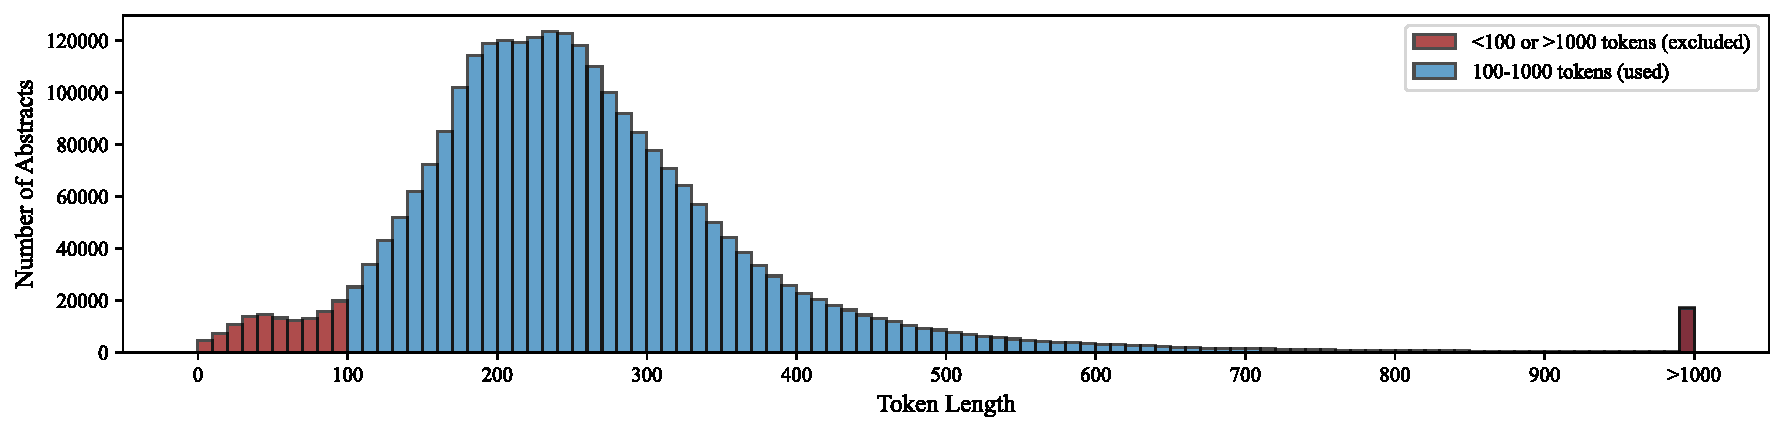
\includegraphics[width=\linewidth]{resources/abstract_token_length_distribution_008.pdf}
	\label{fig:abstract_distribution_histogram}
\end{figure*}



\section{Methodology}

The methodological framework of this study is divided into two complementary domains, directly aligned with the structure of the research questions. 

First, a hierarchical topic modeling approach is applied to the titles and abstracts of all works contained in the curated dataset. The objective of this stage is to algorithmically identify latent subdisciplines within the broader field of artificial intelligence research. By leveraging topic modeling, the study uncovers coherent thematic clusters that reveal the evolving structure of AI subfields as they emerge from textual content.

Second, the study quantifies the relative research authority of individual countries within the subdisciplines identified in the first stage. This is accomplished through a citation-network analysis that computes centrality measures for the most recent research outputs. By constructing directed citation graphs and analyzing their topological properties, the study derives metrics of scholarly influence and connectivity, thereby providing an empirical basis for assessing the international distribution of research leadership in AI.

The following subsections describe these two methodological components in detail.


\subsection{Subdiscipline Retrieval}


The identification of AI subdisciplines is operationalized through a multi-stage hierarchical topic modeling pipeline, combining feature extraction, dimensionality reduction, clustering, and semantic labeling.

To begin, the textual corpus for each work is constructed by appending the title twice to the abstract. This weighting reflects the well-founded assumption that the title is a concise yet highly informative representation of the work’s core contribution, thereby increasing its influence in the embedding space.

For the text vectorization, the \texttt{scikit-learn} \texttt{feature\_extraction} module is employed to transform the preprocessed corpus into high-dimensional embeddings. These embeddings form the basis for subsequent clustering.

A key step in this pipeline is the determination of the number of clusters \(k\). While there exist data-driven heuristics for estimating an ``optimal'' \(k\) (see, e.g., \cite{bulatov2024determination}), the notion that \(k\) is inherent to the data alone is often methodologically fragile and prone to post-hoc rationalization. Consequently, this study adopts a transparent and reproducible approach, treating \(k\) explicitly as a tunable hyperparameter subordinate to the research design.

The principal criterion for selecting \(k\) is practical interpretability and thematic coherence. To this end, UMAP projections are generated to visualize the emergent thematic landscape and to assess the integrity of meaningful clusters. The final \(k\) is chosen to ensure that naturally cohesive thematic areas—such as \textit{Medical AI} and \textit{Education AI}—remain intact without unnecessary fragmentation (e.g., separating \textit{Cancer Diagnosis} and \textit{Medical Image Segmentation}), while ensuring that highly specific research fronts such as \textit{Edge AI} or \textit{Quantum AI} do not dissolve into overly diffuse catch-all clusters.

After clustering, each cluster is assigned an interpretable subdiscipline label. This is accomplished by extracting representative keywords that balance two competing criteria: \textit{Distinctiveness}—terms that differentiate the cluster clearly from others—and \textit{Representativeness}—terms that accurately describe the broader thematic scope of the cluster. This dual criterion ensures that labels do not become overly narrow (overemphasizing idiosyncratic terms) nor overly generic (diluting the thematic specificity), but rather capture the defining characteristics of each subdiscipline in a linguistically meaningful and reproducible manner.

\clearpage
\onecolumn          % leave two-column mode
\begin{center}
	{\large\textbf{Figure~\ref{fig:log_bar_graph}: Topic Modeling Pipeline Diagram}}
	\vspace{1em}
\end{center}

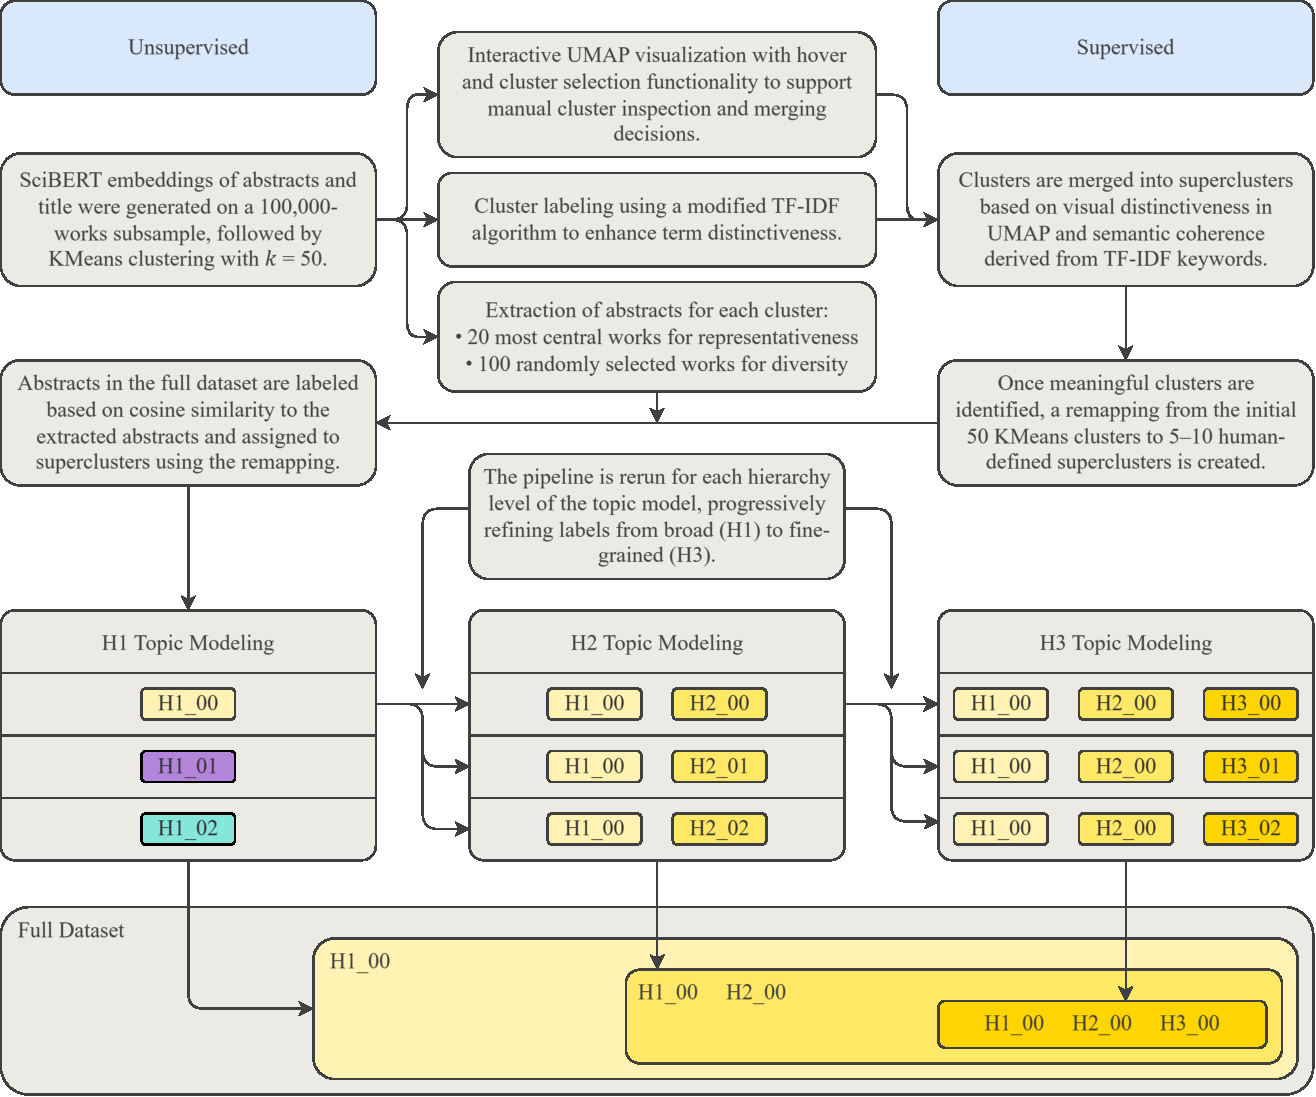
\includegraphics[width=\textwidth]{topic_modeling_pipeline_diagram.pdf}
\label{fig:log_bar_graph}

\twocolumn          % return to two-column mode



\subsection{Quantification of National Research Authority}

To quantify the relative research authority of countries within each identified subdiscipline, a composite impact score was computed for every work in the dataset. This score integrates both traditional citation impact and structural network centrality, weighted to reflect the influence of each publication within its thematic context.

For each work \( p \) in subdiscipline \( s \), the normalized impact score is defined as follows:

\begin{equation}
	\text{Impact}_{p,s} = \alpha \times \text{NormCitations}_{p,s} + \beta \times \text{NormCentrality}_{p,s}
\end{equation}

Here, \(\alpha\) and \(\beta\) are adjustable coefficients that determine the relative contribution of citation counts and network-based authority measures to the overall impact metric.

The normalized citation component is calculated by scaling each paper’s raw citation count relative to the mean citation count of all works published in the same year and subdiscipline:

\begin{equation}
	\text{NormCitations}_{p,s} = 
	\frac{
		\text{Citations}_{p}
	}{
		\text{MeanCitations}_{\text{year},s}
	}
\end{equation}

This normalization corrects for temporal citation accumulation effects and ensures comparability across publication years.

The network-based component, \(\text{NormCentrality}_{p,s}\), is derived from the structural position of each work within the directed citation network. This measure can be operationalized using node-level metrics such as PageRank, which captures both direct and indirect citation flows. The centrality score is then normalized by the maximum or mean value within the respective subdiscipline:

\begin{equation}
	\text{NormCentrality}_{p,s} = 
	\frac{
		\text{Centrality}_{p}
	}{
		\max(\text{Centrality}_{s}) 
		\quad \text{or} \quad
		\text{MeanCentrality}_{s}
	}
\end{equation}

To attribute this impact to countries, each paper’s composite impact score is proportionally distributed according to the institutional affiliations of its authors. The contribution of each country \( c \) is calculated by multiplying the paper’s impact score with the share of authors’ institutions located in that country, as captured by the country distribution vector described in the postprocessing stage.

This procedure produces a subdiscipline-specific authority profile for each country, combining bibliometric performance and network embeddedness with granular affiliation data to yield a robust measure of national research influence within the global AI landsca

\section{Results}

\subsection{Hierarchical Topic Modeling}



%\begin{figure*}[!p]
%	\centering
%	\caption{First Hierarchy of Topic Modeling over 100k Subsample}
%	\vspace{1em}
%	\includegraphics[height=0.95\textheight, keepaspectratio]{mapped_clusters_umap.pdf}
%	\label{fig:L1_hierarchy_topic_modeling}
%\end{figure*}




\subsection{Geomapping of National AI-Authority}

\begin{figure*}[!t]
	\centering
	\caption{Logarithmic distribution of AI-publications by country}
	\vspace{1em}
	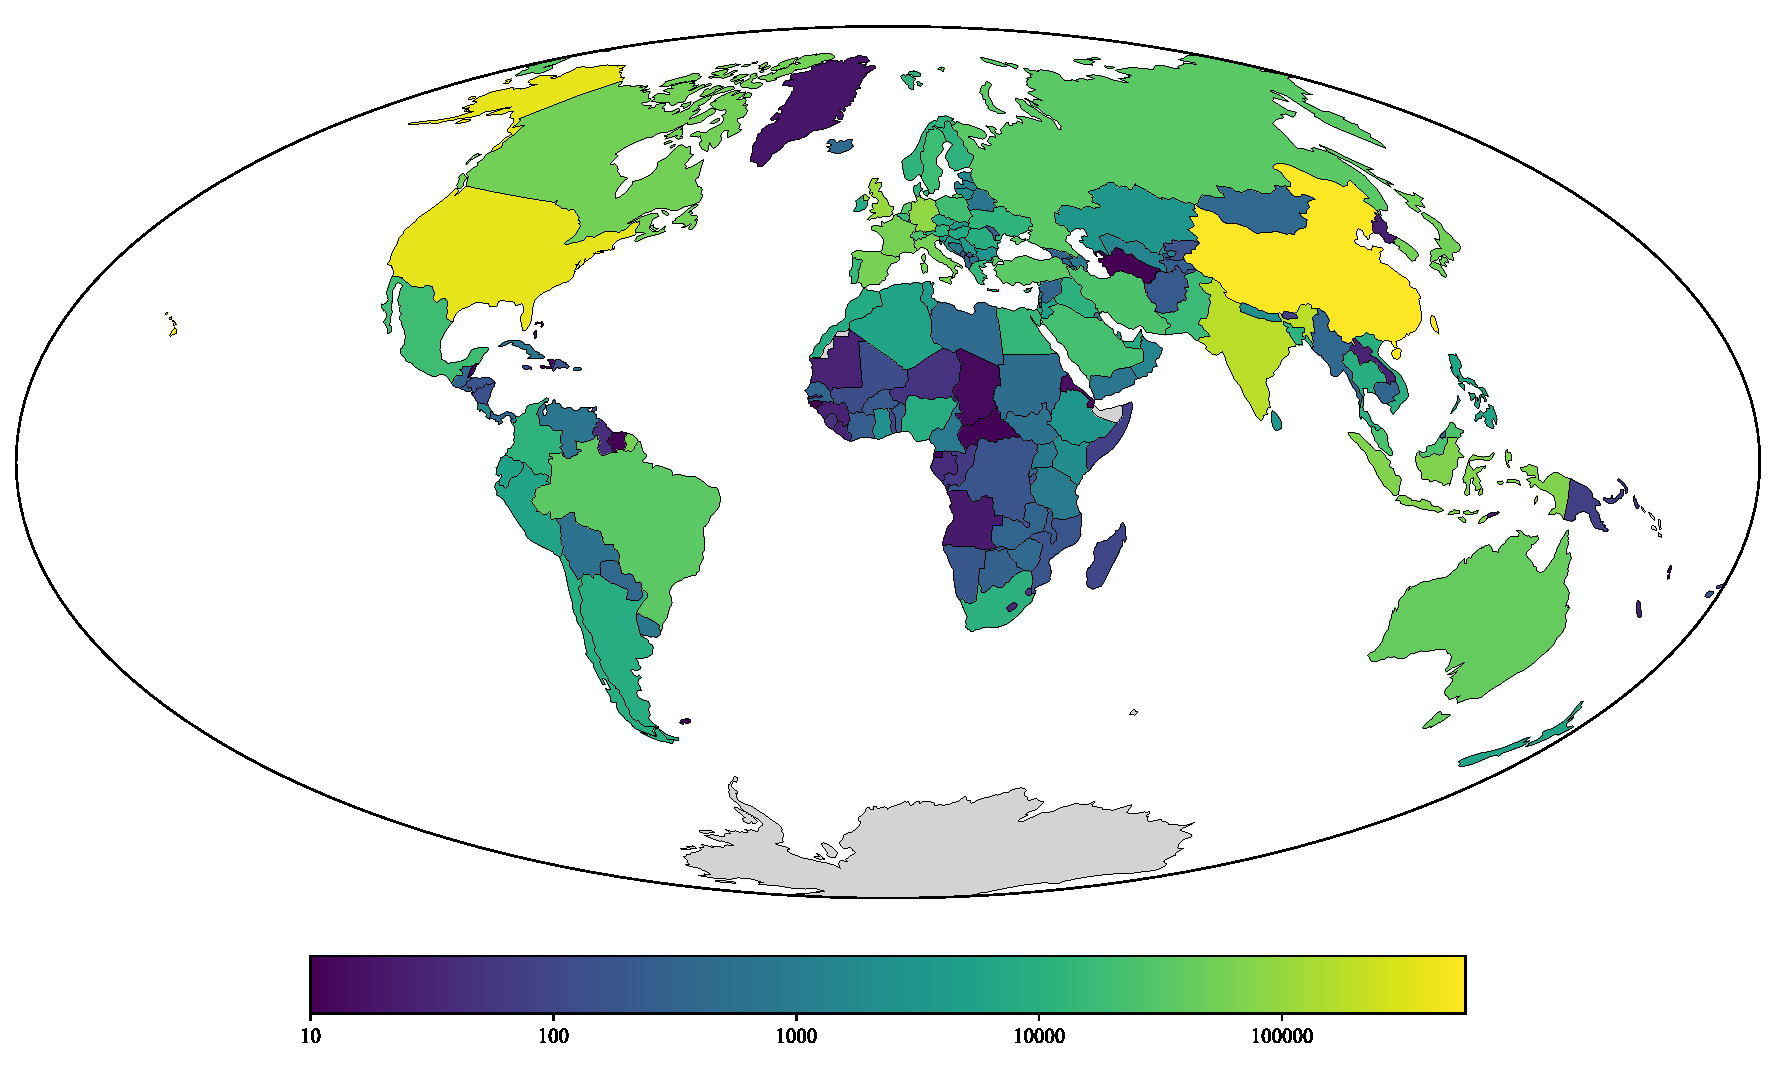
\includegraphics[width=\linewidth]{country_contributions_aitoff_log.pdf}
\end{figure*}

\section{Conclusion}


\section{things i want to add}

-scientometric usually not performed on super recent papers, but here its okay because the dataset is very big AND discipline very focused on newest developments.

-96383209 edges and 22150971 nodes in network of all works

-there is no raw data, patents, publications and every other indicator already for becoming an indicator is prone to distrortion. china is often overproportionate publishing and patenting while bussiness lacks behind.

-caveat section: at the same time us-papers are more cited just for pathdependancy of scientific cooperation not content only.

-at the same time papers have some benefits over other metrics: no inflation-parity calculus, 

-more alarmist introduction: reference ai 2027 paper

-speculation of structural differences: us proprietary, dense models, cn open source sparce and mixture of experts (training on benchmarks and training on api-usecases as one lives from shareholders and the other from market early on)

-filtering method for abstracts: language en, abstract non NULL, country of origin non NULL, abstract more than 99 and less than 1001 tokens.

-the logic behind using both most central and random abstracts in a cluster summary is based on complementarity between representativeness and diversity:

-arbitrary in nature: medial image segmentaiton is BOTH - medical and patter recognition - expert have to decide or choose aesthetic criteria.

-human in the loop-curation: Enables top-down supervision while retaining bottom-up discovery.

- clustes are not mutually-exclusive and jointly-exhaustive, but rather best possible descriptor of cluster (decided by UMAP and tfidf terms). 

- there are domain, field, subfield and topic labels (topic comes first rest is based on that) - but they dont work really well, mainly because model worked on all papers and could be optimized with field specific work (huamn in the loop). also there is a fwci score but fwci doesnt really work for super young paper.

- idea for dominance measurement: how much more citations than expected (median)?

- cluster names were created by looking at the most central abstracts and the tfidf word supplied in the interactive chart.

- caveat: the error stacks up with each hierarchy, even in case of 90 percent percision one would get onle 72.9 percent in a h3 cluster

- words of abstract contain markers for both method and domain - further research - split up into either of those and try to minimise noise by the other.

-quality control maybe testing against the topics from openalex.

- one word can only capture so much - therefore cluster names are often only neighbours to similar issues (example: there are only about 4k paper that are considered tourism - too little to justify its own category, therefore its in the urban development cluster which has the least cosine distance but doesnt reflect that fact). 

- also names can appear twice: geospatial mapping is both a method and an application

- supervision is done on unfiltered umap - no artificial distinctivness enhancement

- density based cluster summarization 

\printbibliography[title={REFERENCES}]

\end{document}